%%%%%%%%%%%%%%%%%%%%%%%%%%%%%%%%%%%%%%%%%%%%%%%%%%%%%%%%%%%%%%%%%%%%%%%%%%%%%%%%
%2345678901234567890123456789012345678901234567890123456789012345678901234567890
%        1         2         3         4         5         6         7         8

\documentclass[letterpaper, 10 pt, conference]{ieeeconf}  % Comment this line out if you need a4paper

%\documentclass[a4paper, 10pt, conference]{ieeeconf}      % Use this line for a4 paper

\IEEEoverridecommandlockouts                              % This command is only needed if 
                                                          % you want to use the \thanks command

\overrideIEEEmargins                                      % Needed to meet printer requirements.

% See the \addtolength command later in the file to balance the column lengths
% on the last page of the document

% The following packages can be found on http:\\www.ctan.org
\usepackage{graphicx} % for pdf, bitmapped graphics files
\usepackage{epsfig} % for postscript graphics files
%\usepackage{mathptmx} % assumes new font selection scheme installed
%\usepackage{times} % assumes new font selection scheme installed
\usepackage{amsmath} % assumes amsmath package installed
\usepackage{amssymb}  % assumes amsmath package installed
\usepackage{algorithm}
\usepackage{algorithmic}

\title{\LARGE \bf
Odometry based on auto-calibrating inertial measurement units attached to the feet
}

\author{Dinesh Atchuthan$^{1}$, Nicolas Mansard$^1$, Joan Sol\`a$^2$% <-this % stops a space
\thanks{$^{1}$ CNRS - LAAS, Toulouse, France, \tt {\small firstname.lastname@laas.fr}}%
\thanks{$^{2}$ IRI, UPC, Barcelona, Spain, \tt{\small jsola@iri.upc.edu}}
}

\begin{document}

\maketitle
\thispagestyle{empty}
\pagestyle{empty}

%%%%%%%%%%%%%%%%%%%%%%%%%%%%%%%%%%%%%%%%%%%%%%%%%%%%%%%%%%%%%%%%%%%%%%%%%%%%%%%%
\begin{abstract}
\end{abstract}


%%%%%%%%%%%%%%%%%%%%%%%%%%%%%%%%%%%%%%%%%%%%%%%%%%%%%%%%%%%%%%%%%%%%%%%%%%%%%%%%
% !TEX root = main.tex

\section{Introduction}\label{sec:intro}

One of the most common ways to describe the trajectory of a body in space is to use odometry, which can be derived from a multitude of sensors, from encoders to GPS and cameras.
The quality of this information is also known to be dependent on the sensor specifications and to accumulate measurement errors. 
The development of SLAM (Simultaneous Localization And Mapping) is mature enough to resolve 
this dependency over time with loop closure strategies. However, other strategies are required to comply with the particularities of legged locomotion and physical interactions in unstructured environments. 
This is particularly necessary in outdoor or industrial applications with cluttered environment. 
In this case, assuming a flat floor is not always reasonable and being able to observe the foot pose allows to implement advanced reactive locomotion strategies.

In the DRC \cite{Johnson:jof:2016,Marion:jof:2017,Karumanchi:jof:2017} most of the teams used laser or RGB-D cameras to build a reconstruction of the floor surface in order to \emph{plan}
the next feet pose. For some teams the level of accuracy was not always sufficient and involved dramatic failures despite intensive training \cite{Kaneko:ichr:2015}.
On the other hand, the IHMC team \cite{Johnson:jof:2016} reported an important gain in terms of accuracy using their state estimator alone,
reaching an impressive $1$\,cm drift per every three steps for the pelvis horizontal position,
and $5$\,mm per every nine steps for the pelvis vertical position. 
Using a quite simple state estimator, it is very interesting to note the following reported factors for reaching this level of precision besides bug fixing:
the redesign of Atlas, coming with a significant reduction of backlash in the leg joints, improving measurements using kinematics and a walking gait reducing the amount of foot slipping and bouncing.
Although the IHMC tested a localization algorithm \cite{Pomerlau:ar:2013}, occasional localization errors were a problem in the overall behavior and SLAM happened to be not necessary in this situation.

\begin{figure}
\centering
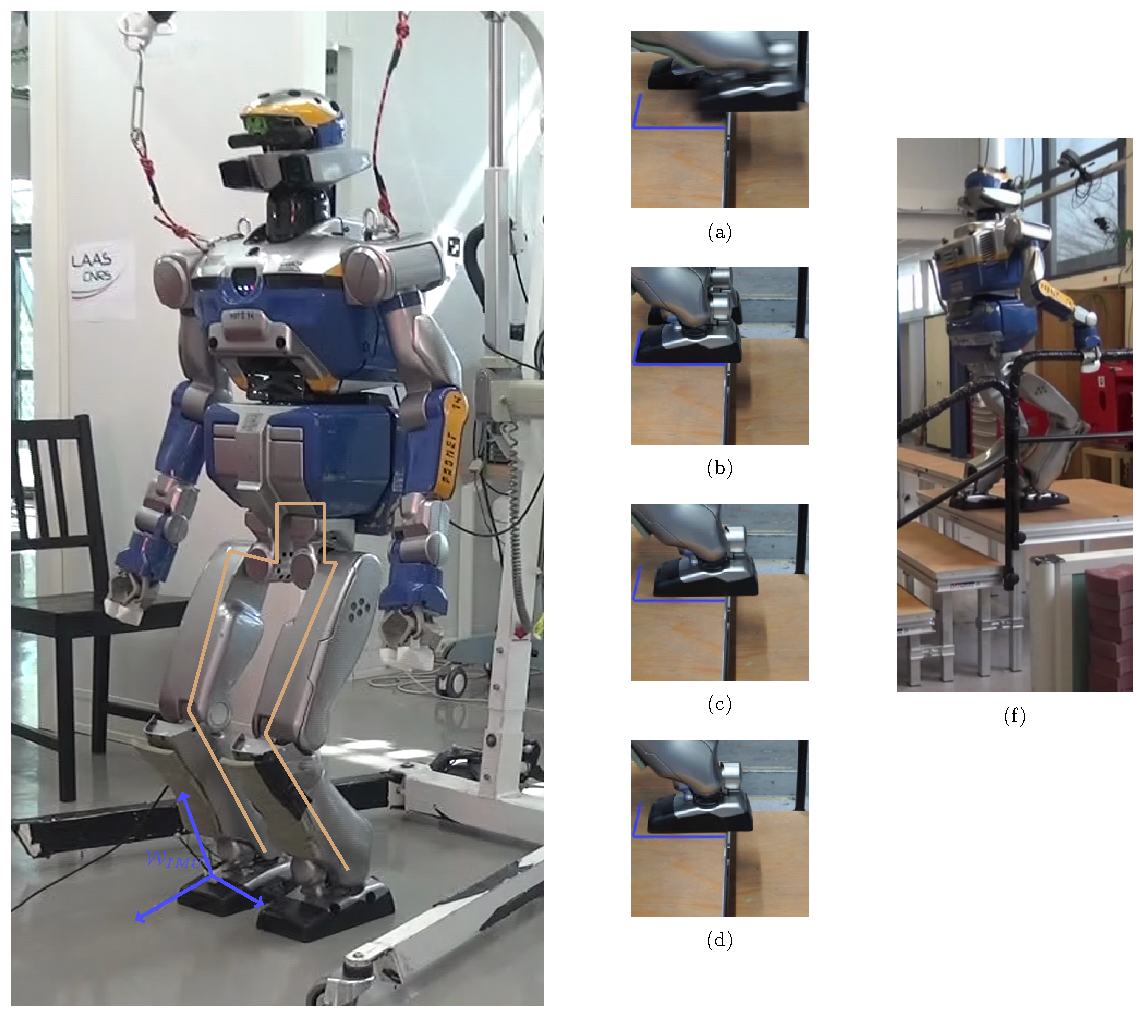
\includegraphics[width=\linewidth]{./figures/cover-figure.pdf}
	\caption{The flying foot trajectory is reconstructed through an IMU set on the foot (in green), and by fusing the information coming from the kinematic chain
        from the support foot to the flying one (in light brown). In the middle images (a)-(d) shows slippage while performing a multicontacts motion depicted on the
        right (e) (from \cite{Carpentier:ICRA:2016}).
 }
	\label{fig:cover}
\end{figure}

For robots where the design choices introduce flexibilities such as HRP-2 \cite{Nakaoka:iros:2007}, or backlashes, the system needs a state estimator being able to take into account this uncertainty.
In addition a good pose estimation of the robot in its environment is still needed for effective interactions with the environment,
and especially for behavior involving manipulation or multiple contact locomotion.
This estimation can then be used to compute the commands that will be sent to actuators.
%<<<<<<< HEAD
%Fusion strategies with information coming from different sensors can be used to achieve this goal. 
%Considering the application in a real environment, we can fuse the odometer with a high frequency proprioceptive sensor 
%to get better predictions of robot poses by improving integration points.
%
%Using an IMU (Inertial Measurement Unit) allows us get acceleration and angular velocity measurement that can be used to 
%compute the pose of the robot and get information similar to odometry by integration for the fusion step.
%These sensors are now used in a wide range of applications: aerospace, SLAM, human motion analysis, or robotics.
%
%=======

Localization can be used to perform real-time planning and model predictive control.
To achieve this goal, fusion strategies with information coming from different sensors is needed.
Graphical methods have been extensively used to implement such fusion strategies \cite{Thrun:ijrr:2006,Kaess:itro:2008}.
They have been used for large modeling estimation problems by means of sparse networks of constraints. 
In robotics, the problems of visual odometry, and simultaneous localization and mapping, have reached a high degree of maturity, 
in great part thanks of the graphical representation. 
This is so, among other aspects, because of the power of the graphical representation to accurately model complex estimation problems. 
These often involve dynamics, proprioceptive measures, exteroceptive measures, and self-calibration.
The graphical representation also allows for the design of powerful nonlinear estimation solvers, which can be built taking into account the needs for accuracy, 
robustness and CPU-performance.
In order to keep the problem tractable and maintain real-time performance a key point is to avoid the graph to be too large for a given time window.
IMUs are challenging in this regards, as their high frequency measurements create large sets of data. 
 
For this reason, \cite{LUPTON-09,forster2015imu} proposed to pre-integrate the IMU information over an horizon where IMU data are the only
ones to be measured.
A first contribution of this paper is to reformulate the method proposed in \cite{forster2015imu} from rotation matrix to quaternion representation
and give a detailed and simpler algebraic derivation.
The second contribution is to apply this method to the measurement of a humanoid robot flying foot pose.
The level of accuracy obtained with this approach allows us to detect foot slippage. 
Finally, we describe the implementation of this pre-integration scheme in a software implementation of the graphical method.
%>>>>>>> 8a2771fa9c6aae6c3980ef5238504b80af3260c9





% !TEX root = main.tex

\section{Experiments} \label{sec:experiments}

The confidence one can have on the encoders of the robot depends on several factors from actuators design to control strategies. in the legged locomotion case, this can also depend on the general design of the robot.
Thus during walking phases with humanoid robot HRP2, one can notice sliding phenomenon when the foot hits the ground. If this effect is not measured, their occurrences can turn to be a problem for navigation in unstructured environment. 
Furthermore, we cannot anticipate the sliding, meaning that we do not know what actually causes this to happen. 
In this context, we show that measuring this slide and getting a better estimation of both real trajectories and real position of the foot is possible with an IMU fixed on the sliding member, the foot of the robot in our case.

In order to get to that point, we first want to check whether our fusion method of both IMUs and odometer is able to get a correct estimation of one's foot during walking.
Then we show that using an IMU on the foot of the robot leads to a better estimation of the real position of the member compared to encoder based odometry.

We chose to use a low-cost IMU in our application to realize the feasibility of our method. For this purpose we selected the 
MPU6050 from Invensense combining both an accelerometer and a gyroscope and extensively used in the open source community.


%\textit{Keywords : low-cost IMU, MPU6050, experiment conditions, 1 KHz IMU} \\
%\textit{TODO : add factor graph for experiment visualization}

\subsection{Method}
\subsubsection{auto-calibration}

The parameters we need to calibrate for a correct integration are the biases on top of which we integrate the incoming data of the IMU.
The time varying property of the bias is a critical point to consider in order to avoid large deviations. This calibration is made possible
by dependencies of the delta pre-integration ($\boldsymbol{\Delta P}(ab, \omega b), \boldsymbol{\Delta V}(ab, \omega b), \boldsymbol{\Delta Q}(\omega b)$). Fusing both odometer and IMU provides constraints on position and orientation parts of
the state vector. However, velocity is still not observable and is affected by the bias estimation. In the case of legged locomotion, we fix the observability problem by adding a zero velocity constraint when the foot is on the ground.

The initial orientation estimation is made possible by adding an absolute constraint on yaw part of the state vector, otherwise we would run in observability problems. \textbf{add figure here (graph)}

\subsection{Results}
\subsubsection{Trajectory reconstruction}

We check the feasibility of the trajectory reconstruction using a 1Khz IMU attached to one's foot tracked with a motion capture (MOCAP) system. The MOCAP is used to get odometry between zero-velocity phases, i.e. when the foot is on the ground,
and will be taken as the ground truth against which we compare the trajectory reconstruction.

We reproduce the movements the feet of a robot could have when it is walking. However, as shown in figures \textbf{add figure here}, the final optimal state
is not the expected one and acceleration biases are rapidly changing. The variation that we can see is not only due to some random walk and can be explained by the excitement of biases in a different axis.
As explained in \cite{roussillon2011rt}, in opposition to gyroscope biases, acceleration biases do not converge toward stable values during a motion exciting several axis of the sensor. 
This effect can be explained by time inconsistency meaning that we fail
to use the information of the entire motion to converge toward stable values as expected in the sensor model, but the problem may also be that the step motions do not use all the axis of the accelerometer as it should.

We fix the trajectory estimation problem by adding odometry information during foot's flying phase. However, we cannot fix any other conditions making velocity and bias observation possible hence all parameters of the state vector are estimated.
This added KeyFrame reduces the integration time since last state optimization making bias random walk variation less critical on estimation. As we can see, results are much better and closer to MOCAP's ground truth as we could expect.

%TODO : process mocap experiments

\subsubsection{Legged-Locomotion's undesired behavior measurement}

We use the approach presented above in the case of the humanoid robot HRP2 to better estimate the trajectory of the foot. This also results in a better estimation of the pose of the robot using its kinematic chain. 
For this experiment, the robot is moving in open loop and some particularities are worth to be noted compared to previous experiment. 
The structure of the robot produces vibrations that are measured by the IMU, thus explaining the over noisy aspect of the data. The foot's flying phase is set to last 800 ms. The double support phase lasts only 20 ms, thus it is difficult to observe
even with the IMU working at 1 KHz because of the vibration it will measure on impacts.




%TODO experiment : step motion + complex rotation, followed by MOCAP



% !TEX root = main.tex

\section{Conclusion}

We have presented a method to measure foot movement during robot biped locomotion. We fuse information from an IMU attached to the foot, the kinematic chain measured by the robot encoders, and available knowledge extracted from the gait phases, such as zero velocity and IMU bias dynamics. We used nonlinear optimization techniques based on factor graphs, which has proved to be a flexible and powerful fusion framework. For this, we have revised the IMU pre-integration theory, and proposed an implementation in the quaternions manifold, with simpler derivations than previous works, and with physical interpretations, which we believe go in the direction of improving the clarity of the method.


Results showed that this estimation method is able to detect subtle movements that are not measurable using the encoders alone, such as a sliding foot condition at the beginning or end of the contact phase. These slides, if undetected, have a dramatic negative impact on the overall robot odometry.

%%%%%%%%%%%%%%%%%%%%%%%%%%%%%%%%%%%%%%%%%%%%%%%%%%%%%%%%%%%%%%%%%%%%%%%%%%%%%%%%
%\section*{ACKNOWLEDGMENT}
%Work sponsored by FP7 EUROC, ANR LOCO3D and?

%%%%%%%%%%%%%%%%%%%%%%%%%%%%%%%%%%%%%%%%%%%%%%%%%%%%%%%%%%%%%%%%%%%%%%%%%%%%%%%%
\bibliographystyle{IEEEtran}
\bibliography{IEEEabrv,bib}

\end{document}
